\documentclass[11pt]{article}

\usepackage[a4paper,margin=1in]{geometry}
\usepackage{amsmath, amssymb, mathtools}
\usepackage{tikz}
\usetikzlibrary{calc}
\usepackage{pgfplots}
\pgfplotsset{compat=1.18}
\usetikzlibrary{positioning, arrows.meta, shapes.geometric}
\usepackage{xcolor}
\definecolor{DollarColor}{RGB}{107, 128, 104}
\definecolor{EuroColor}{RGB}{93, 126, 167}
\definecolor{BitcoinColor}{RGB}{247, 147, 26}
\usepackage{minted}
\usepackage{siunitx}
\usepackage{booktabs, array, tabularx}
\usepackage[linesnumbered,ruled,vlined]{algorithm2e}
\usepackage{hyperref}

\begin{document}

\title{Fast Arbitrage Detection}
\author{Claudio Raimondi}
\date{\today}
\maketitle

\begin{abstract}
Triangular arbitrage offers opportunities to exploit price inefficiencies between three currency pairs. While several algorithms exist for triangular arbitrage detection, their computational efficiency and accuracy can vary. In this report, I present a straight forward method that combines logarithmic properties with numerical representation techniques and advanced parallelization strategies to accurately and efficiently detect arbitrage opportunities.
\end{abstract}

\tableofcontents

\section{Introduction}
The process to exploit triangular arbitrage opportunities involves 3 generic steps, each crucial for ensuring the success of the strategy:
\begin{enumerate}
    \item \textbf{Data Collection:} Gather real-time exchange rates for the currency pairs involved.
    \item \textbf{Data Manipulation:} Use the collected data to detect profitable trades.
    \item \textbf{Execution:} Execute trades to lock in profits.
\end{enumerate}
For all three steps, the \textbf{speed} and \textbf{accuracy} of the algorithm are paramount. All the efforts become vain if somebody else collets, manipulates, and executes the arbitrage opportunity before you do.
On this report, I will focus on the \textbf{second step}---\textit{data manipulation}---, which is the most short-lived. The other two steps rely on external factors, such as networks and exchange APIs.

\section{Visualization}
To visualize triangular arbitrage, we can represent it as a \textbf{directed graph} (more precisely a clique), where each node represents a currency and each edge represents an exchange rate.

\begin{center}
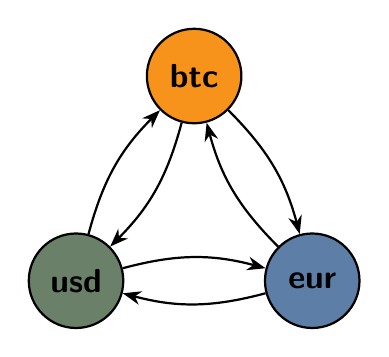
\begin{tikzpicture}[>=Stealth, thick, main/.style={draw, circle, minimum size=1.2cm, font=\sffamily\large\bfseries}]

\coordinate (A) at (0,0);
\coordinate (B) at (3,0);
\coordinate (C) at ($(A)!0.5!(B) + (0,2.6)$);

\node[main, fill=DollarColor]  (usd) at (A) {usd};
\node[main, fill=EuroColor]    (eur) at (B) {eur};
\node[main, fill=BitcoinColor] (btc) at (C) {btc};

\draw[->] (usd) to[bend left=15] node[above] {} (eur);
\draw[->] (eur) to[bend left=15] node[above] {} (btc);
\draw[->] (btc) to[bend left=15] node[above] {} (usd);

\draw[->] (eur) to[bend left=15] node[above] {} (usd);
\draw[->] (btc) to[bend left=15] node[above] {} (eur);
\draw[->] (usd) to[bend left=15] node[above] {} (btc);

\end{tikzpicture}
\end{center}

\section{Arbitrage Formula}

\subsection{Base Formula}
The formula to detect a profitable triangular arbitrage path, given three exchange rates $R$, is the following inequality:
\begin{equation}
    R_{1} \cdot R_{2} \cdot R_{3} > 1
\end{equation}

\subsection{Price Format}
If the \textit{data collection} layer is serious about efficiency and precision, the prices are provided in \textbf{fixed point} representation as a combination of \textbf{mantissa} and \textbf{exponent} such that $R = m \cdot 10^{e}$. So the formula becomes:

\begin{equation}
    \left( m_1 \cdot 10^{e_1} \right) \cdot \left( m_2 \cdot 10^{e_2} \right) \cdot \left( m_3 \cdot 10^{e_3} \right) > 1
\end{equation}
\begin{equation}
    m_1 \cdot m_2 \cdot m_3 \cdot 10^{e_1 + e_2 + e_3} > 1
\end{equation}
\begin{equation}
    m_1 \cdot m_2 \cdot m_3 > \frac{1}{10^{e_1 + e_2 + e_3}}
\end{equation}
\begin{equation}
    m_1 \cdot m_2 \cdot m_3 > 10^{-(e_1 + e_2 + e_3)}
\end{equation}

\subsection{Logarithmic Form}
In most computer systems, where registers are limited to 64 bits, the product of three mantissas can easily overflow. To address this, we can use logarithmic properties to transform the \textbf{product} into an \textbf{addition} of much smaller numbers and the \textbf{power} into a \textbf{product}:
\begin{equation}
    \log_b(m_1 \cdot m_2 \cdot m_3) > \log_b(10^{-(e_1 + e_2 + e_3)})
\end{equation}
\begin{equation}
    \log_b(m_1) + \log_b(m_2) + \log_b(m_3) > -(e_1 + e_2 + e_3) \cdot \log_b(10)
\end{equation}

\subsection{Inverse Direction}
As of now, we have only considered the \textbf{forward direction} of the triangular arbitrage, i.e. the forward cycle path. But since the rates are bidirectional, we can also exploit price inefficiencies in the \textbf{reverse direction}. Assuming we don't have the rates for the reverse direction, we can compute them as the inverse of the forward rates, and the formula becomes:
\setcounter{equation}{0}
\begin{equation}
    \frac{1}{R_{1}} \cdot \frac{1}{R_{2}} \cdot \frac{1}{R_{3}} > 1
\end{equation}
\begin{equation}
    \frac{1}{R_{1} \cdot R_{2} \cdot R_{3}} > 1
\end{equation}
\begin{equation}
    R_{1} \cdot R_{2} \cdot R_{3} < 1
\end{equation}
\begin{equation}
    \log_b(m_1) + \log_b(m_2) + \log_b(m_3) < -(e_1 + e_2 + e_3) \cdot \log_b(10)
\end{equation}
As expected, the only difference is the direction of the inequality. This means that at any time there always exists a profitable arbitrage opportunity, either in the forward or reverse direction (unless the market is perfectly efficient). However in practice, not every opportunity is worth exploiting, wether due to \textbf{fees} or the \textbf{spread}\textsuperscript{\cite{spread}}.

\subsection{The Spread Problem}
At first, the two inequalities seem to differ only in the direction of the inequality. However, in practice, the two inequalities are not equivalent. In fact, due to the \textbf{spread}, we need to use different exchange rate values based on the direction of the trade. Specifically, we need to use the \textbf{ask prices} when buying and the \textbf{bid prices} when selling. So the inequalities become:
\setcounter{equation}{0}
\begin{equation}
    \log_b(m_{\text{bid}_1}) + \log_b(m_{\text{bid}_2}) + \log_b(m_{\text{bid}_3}) > -(e_1 + e_2 + e_3) \cdot \log_b(10)
\end{equation}
\begin{equation}
    \log_b(m_{\text{ask}_1}) + \log_b(m_{\text{ask}_2}) + \log_b(m_{\text{ask}_3}) < -(e_1 + e_2 + e_3) \cdot \log_b(10)
\end{equation}

\subsection{Threshold}
Often times, to avoid false positives and very short-lived arbitrage opportunities, we need to set a profitability \textbf{threshold}. This threshold is a percentage value that represents the minimum profit we want to achieve from the arbitrage opportunity and allows us to filter out the noise.
Let $\tau$ be the threshold as a decimal (e.g., $0.001$ for $0.1\%$). Then the adjusted arbitrage inequalities become:
\setcounter{equation}{0}
\begin{equation}
    \log_b(m_{\text{bid}_1}) + \log_b(m_{\text{bid}_2}) + \log_b(m_{\text{bid}_3}) > -(e_1 + e_2 + e_3) \cdot \log_b(10) + \log_b(1 + \tau)
\end{equation}
\begin{equation}
    \log_b(m_{\text{ask}_1}) + \log_b(m_{\text{ask}_2}) + \log_b(m_{\text{ask}_3}) < -(e_1 + e_2 + e_3) \cdot \log_b(10) - \log_b(1 + \tau)
\end{equation}

\section{Algorithm}

\subsection{The choice of the base}
Up to this point, we have considered the base $b$ of the logarithm to be arbitrary. But in practice, we have to choose the one that best fits our needs.
\begin{itemize}
    \item $\log_{10}$ allows for a simplification of the formula: $\log_{10}(10) = 1$.
    \item $\log_{2}$ can be computed with fast bit-shifts, and it is the natural choice for binary systems\textsuperscript{\cite{bithacks}}.
\end{itemize}
In this implementation, I chose the latter. This decision is motivated by both \textbf{efficiency} and \textbf{precision} gains. In fact the logarithm base 2 has some unique properties:
\begin{itemize}
    \item the integer part corresponds to 63 minus the number of leading zeros in the binary representation of the value.
    \item since floating point numbers are naturally represented in base 2, there is virtually no loss of precision.
\end{itemize}
Furthermore, the small advantage of using base 10 becomes irrelevant since we can precompute the value of $\log2(10)$ anyways.

\subsection{Precomputation}
Assuming exponents change very rarely, we can use an optimistic approach and \textbf{precompute} the entire right side of the inequality, storing it in a constant variable, raising an exception or even updating the precomputed constant only when the exponents change.

\subsection{Fixed Point Representation}
Since the logarithm produces a real number, I will use a \textbf{fixed point} representation to store the result. This allows for much faster additions and comparisons compared to floating point numbers. For reference, a float add takes about 4-5 cycles on modern CPUs\textsuperscript{\cite{agner2024}}, while a fixed point addition takes only 1 cycle. Specifically, since the maximum possible value of the logarithm is $log_2(2^{63}) = 63$ and our formula sums three of them together, we need $\lceil \log_2(64 * 3) \rceil = 8$ bits to store integers up to 192. The fractional part can be chosen based on the desired precision. At this point we have three options for the fixed point format:
\begin{itemize}
    \item Q8.8 as 16 bits $\rightarrow 2^{-8} = 0.00390625$ step size.
    \item Q8.24 as 32 bits $\rightarrow 2^{-24} = 0.00000006$ step size.
    \item Q8.56 as 64 bits $\rightarrow 2^{-56} = 0.000000000000000014$ step size.
\end{itemize}
Out of the three, the second option offers the best balance between precision and size. For instance, a maximum error of $\text{step\_size} / 2 = 0.0.00000006 / 2 = 0.00000003$ in the logarithmic value corresponds to a relative error of $2^{0.00000003} - 1 \approx 2.1 \cdot 10^{-8} = 0.0000021\%$ in the original value, which is more than enough precision for our needs.

\subsection{Log2}
The actual implementation of the \texttt{log2} function relies on the \textbf{clz} (count leading zeros) intrinsic for the integer part, and a \textbf{lookup table} for the fractional part. The table is generated by sampling the logarithm function at regular intervals in the range $[0, 1]$.
The \textbf{table size} directly influences the precision of the fractional part. Specifically, it determines the number of samples taken in the $[0, 1]$ range along the horizontal axis of the logarithm function.
\begin{table}[h]
\centering
\begin{tabular}{|c|c|c|c|}
\hline
\textbf{TABLE\_SIZE} & \textbf{Memory Usage} & \textbf{Horizontal Step Size} & \textbf{Vertical Step Size (approx.)} \\
\hline
256     & 1 KB    & $0.00391$   & $\sim0.00026$ \\
512     & 2 KB    & $0.00195$   & $\sim0.00013$ \\
1024    & 4 KB    & $0.00098$   & $\sim0.000068$ \\
\hline
\end{tabular}
\caption{Trade-offs between memory usage and precision for various table sizes}
\end{table}

A lookup table with \textbf{256 entries} is the best compromise between precision and memory usage. In fact, this brings down the step size from $0.00000006$ to $0.00026$, or a maximum error of $0.00026 / 2 = 0.00013$, which corresponds to a relative error of $2^{0.00013} - 1 \approx 9 \cdot 10^{-5} = 0.009\%$ in the original value. This is a perfectly reasonable trade-off, considering that most arbitrage opportunities are above the $0.1\%$ threshold. Furthermore, the error does not accumulate, since the additions that would follow in our formula are all performed on the fixed point numbers discussed earlier, which have a much greater margin of error. Considering that modern CPUs have \textbf{L1 caches} of at least 32 KB, a 1 KB lookup table will most likely always be present in the cache, making the lookup operation extremely fast

\newpage
\begin{minted}[fontsize=\footnotesize, xleftmargin=1em, linenos=false]{cpp}
template <uint8_t IntBits, uint8_t FracBits = 32 - IntBits>
constexpr FixedPoint<IntBits, FracBits> FixedPoint<IntBits, FracBits>::log2(const uint64_t value)
{
  static constexpr uint32_t TABLE_BITS = std::min(8, FracBits); //2^8 = 256 entries
  static constexpr uint32_t TABLE_SIZE = 1 << TABLE_BITS;
  static constexpr uint32_t SHIFT_AMOUNT = 63 - TABLE_BITS;
  static constexpr uint32_t MASK = TABLE_SIZE - 1;

  static constexpr std::array<uint32_t, TABLE_SIZE> log2_table = precomputeLog2Table<TABLE_SIZE>();

  const uint64_t leading_zeroes = __builtin_clzll(value);
  const uint32_t integer_part = 63 - leading_zeroes;
  const uint64_t shifted = value << leading_zeroes;
  const uint32_t table_index = (shifted >> SHIFT_AMOUNT) & MASK;
  const uint32_t frac_part = log2_table[table_index];

  const int32_t raw_value = (static_cast<int32_t>(integer_part) << FracBits) + frac_part;
  return FixedPoint<IntBits, FracBits>::fromRaw(raw_value);
}
\end{minted}
In this implementation the \textbf{zero check} is avoided to prevent unnecessary \textbf{branching}. Since the logarithm of zero is undefined, it is safe and coherent to leave it undefined behavior. After all these considerations, this function is able to compile in just $\sim{10}$ instructions, which is 3x faster than optimized standard log2 implementations\textsuperscript{\cite{libc_log2}}.

\section{Parallelization}
% parallelization (either of the bellman-ford or of the 2 formulas (6 logs in parallel))

\begin{thebibliography}{9}

\bibitem{spread}
Wikipedia, \textit{Bid–ask spread}, Available at: \url{https://en.wikipedia.org/wiki/Bid%E2%80%93ask_spread}.
\bibitem{agner2024}
Agner Fog, \textit{Instruction Tables: Lists of instruction latencies, throughputs and micro-operation breakdowns}, 2024. Available at: \url{https://www.agner.org/optimize/instruction_tables.pdf}.
\bibitem{bithacks}
Sean Eron Anderson, \textit{Bit Twiddling Hacks}, 2005. Available at: \url{https://graphics.stanford.edu/~seander/bithacks.html}.
\bibitem{libc_log2}
GNU C Library, \textit{log2}, 2023. Available at: \url{https://github.com/bminor/glibc/blob/master/sysdeps/ieee754/dbl-64/e_log2.c}.

\end{thebibliography}

\end{document}
